% MASTER 2 -- Scaled nMOS transistor (cross-section), original vs scaled.
% Covers Q6 ("draw scaled nMOS transistor"). All linear dims divide by alpha;
% gate-oxide thickness D and supply V_DD divide by beta (beta=alpha -> constant field,
% beta=1 -> constant voltage). The same cross-section, drawn smaller, is the whole idea.
\documentclass[border=10pt]{standalone}
\usepackage{amsmath}
\usepackage{tikz}
\usetikzlibrary{arrows.meta}
\begin{document}
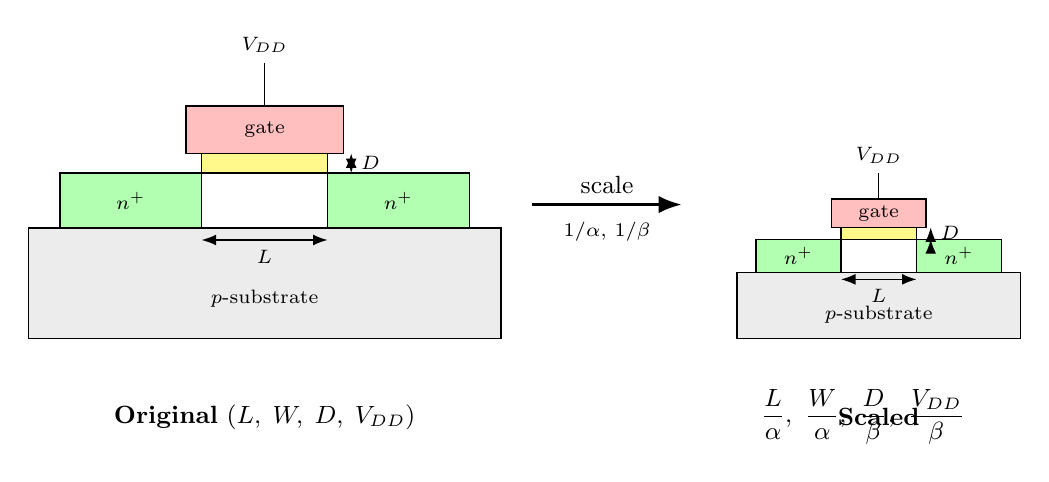
\begin{tikzpicture}[>=Latex,font=\small,line width=0.5pt]
% one device drawn from local origin (0,0); coords span x:0..6, y:0..3.5
\newcommand{\dev}{%
  \fill[gray!15] (0,0) rectangle (6,1.4);                 % p-substrate
  \node at (3,0.5) {\scriptsize $p$-substrate};
  \fill[green!30] (0.4,1.4) rectangle (2.2,2.1);          % n+ source
  \fill[green!30] (3.8,1.4) rectangle (5.6,2.1);          % n+ drain
  \node at (1.3,1.75) {\scriptsize $n^+$};
  \node at (4.7,1.75) {\scriptsize $n^+$};
  \fill[yellow!45] (2.2,2.1) rectangle (3.8,2.35);        % gate oxide
  \fill[red!25] (2.0,2.35) rectangle (4.0,2.95);          % gate (poly)
  \node at (3,2.65) {\scriptsize gate};
  \draw (0,0) rectangle (6,1.4);
  \draw (0.4,1.4) rectangle (2.2,2.1);
  \draw (3.8,1.4) rectangle (5.6,2.1);
  \draw (2.2,2.1) rectangle (3.8,2.35);
  \draw (2.0,2.35) rectangle (4.0,2.95);
  \draw[<->] (2.2,1.25) -- (3.8,1.25) node[midway,below]{\scriptsize $L$}; % channel length
  \draw[<->] (4.10,2.10) -- (4.10,2.35) node[midway,right]{\scriptsize $D$}; % oxide thickness
  \draw (3,2.95) -- (3,3.5) node[above]{\scriptsize $V_{DD}$};            % supply
}
% --- original device ---
\begin{scope}
  \dev
  \node at (3,-1.0) {\textbf{Original} ($L,\;W,\;D,\;V_{DD}$)};
\end{scope}
% --- scaled device (all coords x0.6) ---
\begin{scope}[xshift=9cm,scale=0.6]
  \dev
  \node at (3,-1.0/0.6) {\textbf{Scaled}};
\end{scope}
\node[align=center] at (10.6,-1.0)
  {$\dfrac{L}{\alpha},\ \dfrac{W}{\alpha},\ \dfrac{D}{\beta},\ \dfrac{V_{DD}}{\beta}$};
% scaling arrow
\draw[->,very thick] (6.4,1.7) -- (8.3,1.7) node[midway,above]{scale};
\node at (7.35,1.35) {\scriptsize $1/\alpha,\,1/\beta$};
\end{tikzpicture}
\end{document}
